\documentclass[../main.tex]{subfiles}
\begin{document}
\chapter{Permutations}
\section{Introduction to Permutations}
Recall that a permutation of a set $X$ is a bijection from $X \to X$ and that $\Sym(X)$ is the group of all such permutations.
\begin{example}
  \label{permutationExample}
  $X = \{1, 2, 3\}$, $\Sym X \cong S_3$
  \begin{center}
  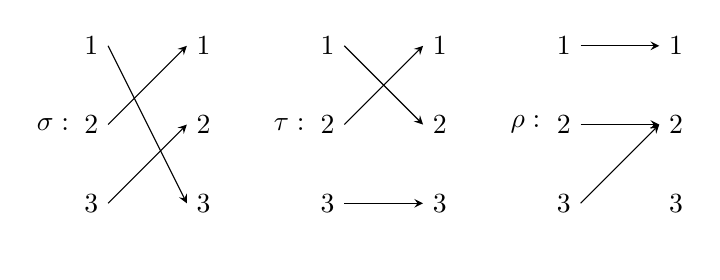
\begin{tikzpicture}[>=stealth]
    \node at (-0.7, 0) {$\sigma:$};
    \draw[->] (0, 1) node[left] {1} -- (1, -1) node[right] {3};
    \draw[->] (0, 0) node[left] {2} -- (1, 1) node[right] {1};
    \draw[->] (0, -1) node[left] {3} -- (1, 0) node[right] {2};
    \node at (0.5, -1.5) {\tick};
    \begin{scope}[xshift=3cm]
      \node at (-0.7, 0) {$\tau:$};
      \draw[->] (0, 1) node[left] {1} -- (1, 0) node[right] {2};
      \draw[->] (0, 0) node[left] {2} -- (1, 1) node[right] {1};
      \draw[->] (0, -1) node[left] {3} -- (1, -1) node[right] {3};

      \node at (0.5, -1.5) {\tick};
    \end{scope}
    \begin{scope}[xshift=6cm]
      \node at (-0.7, 0) {$\rho:$};
      \draw[->] (0, 1) node[left] {1} -- (1, 1) node[right] {1};
      \draw[->] (0, 0) node[left] {2} -- (1, 0) node[right] {2};
      \draw[->] (0, -1) node[left] {3} -- (1, 0);
      \node[right] at (1, -1) {3};
      \node at (0.5, -1.5) {\cross};
    \end{scope}
  \end{tikzpicture}
  \end{center}
  Here, $\sigma$ and $\tau$ are permutations as they are bijective, however, $\rho$ is not as it is not a bijection.

  We can compute composition of permutations using diagrams:
  \begin{center}
  \begin{tikzpicture}
    \node at (0.75, 1.5) {$\sigma$};
    \draw[|->] (0, 1) node[left] {1} -- (1.5, 1) node[right] {3};
    \draw[|->] (0, 0) node[left] {2} -- (1.5, 0) node[right] {1};
    \draw[|->] (0, -1) node[left] {3} -- (1.5, -1) node[right] {2};

    \begin{scope}[xshift=2cm]
      \node at (0.75, 1.5) {$\tau$};
      \draw[|->] (0, 1) -- (1.5, 1) node[right] {3};
      \draw[|->] (0, 0) -- (1.5, 0) node[right] {2};
      \draw[|->] (0, -1) -- (1.5, -1) node[right] {1};
    \end{scope}
  \end{tikzpicture}
  \end{center}
  Because we applied $\sigma$ first and then $\tau$, we write $\tau \sigma$ as it is a composition of functions.
  Drawing diagrams like this is quite cumbersome so we will introduce notation to simplify this.
\end{example}
\subsection{Cycles}
\begin{definition}
  Any list of $k$ \textbf{distinct} elements $a_1, \ldots, a_k \in \{1, \ldots, n\}$ determines a \textit{$k$-cycle}.
  \[
    \sigma = \cycle{a_1 a_2 {\cdots} a_n}
  \]
  as follows:
  \[
    \sigma(b) = \begin{cases}
    a_{i + 1} & \text{ if }b = a_i,\ i < k \\
    a_1 & \text{ if }b = a_k \\
    b & \text{ otherwise}
    \end{cases}
  \]
\end{definition}
\begin{example}
  For the permutations as in \cref{permutationExample}
  \[
    \sigma = \cycle{1 3 2} = \cycle{3 2 1} \text{ and } \tau = \cycle{1 2}
  \]
\end{example}
With practice, you can get proficient at multiplying cycles.
The most important thing to ensure that you \textbf{start from the right}.
\begin{example}
  Using the same permutations again:
  \[
    \tau \sigma = \cycle{1 2}\cycle{1 3 2} = \cycle{1 3}
  \]
  \begin{itemize}
    \item We start by writing 1.
    \item Now check where 1 goes.
      In the first cycle, $1 \mapsto 3$.
      In the second cycle 3 is unchanged.
      So we write 3.
    \item Now we check where 3 goes.
      In the first cycle $3 \mapsto 2$.
      In the second cycle $2 \mapsto 1$.
      We have already written 1 so we are done.
  \end{itemize}
  A more difficult example:
  \[
    \cycle{1 4 3 2}\cycle{2 4 3} = \cycle{1 4 2 3}
  \]
  \begin{itemize}
    \item We start by writing 1.
    \item Now check where 1 goes.
      In the first cycle 1 is unchanged.
      In the second cycle $1 \to 4$.
      So we write 4.
    \item Now check where 4 goes.
      In the first cycle $4 \mapsto 3$.
      In the second cycle $3 \mapsto 2$.
      So we write 2.
    \item Now check where 2 goes.
      In the first cycle $2 \mapsto 4$.
      In the second cycle $4 \mapsto 3$.
      So we write $3.$
    \item Now we check where 3 goes.
      In the first cycle $3 \mapsto 2$.
      In the second cycle $2 \mapsto 1$
      We have already written 1 so we are done.
  \end{itemize}
\end{example}
\begin{remark} Cyclically permuting elements in a cycle does not change the cycle.

  That is:
  \[
    \cycle{a_1 a_2 a_3 {\cdots} a_k} = \cycle{a_2 a_3 {\cdots} a_k a_1} = \cycle{a_3 {\cdots} a_k a_1 a_2}
  \]
  and so on.
\end{remark}
\begin{definition}[Disjoint Cycles]
  Cycles $\cycle{a_1 {\cdots} a_k}$ and $\cycle{b_1 {\cdots} b_k}$ are \textit{disjoint} if $a_i \neq b_j$ for all $i, j$.
\end{definition}
\begin{remark}[Warning]
  In general, cycles \textbf{do not commute}, however disjoint cycles always \textbf{commute}.
\end{remark}
\begin{theorem}[Disjoint Cycles]
  Every $\sigma \in S_n$, can be written as a product of disjoint cycles.

  This expression is unique, up to:
  \begin{itemize}
    \item Shifting elements within a cycle.
    \item Reordering the cycles (as they commute).
  \end{itemize}
\end{theorem}
\begin{proof}
  The action of the subgroup $\langle \sigma \rangle$ on $X = \{1, \ldots, n\}$ partitions $X$ into orbits:
  \[
    X = \langle \sigma \rangle i_1 \cup \langle \sigma \rangle i_2 \cup \cdots \cup \langle \sigma \rangle i_k
  \]
  \textbf{Existence}\par
  Let $n_j = |\langle \sigma \rangle i_j|$.
  We see that:
  \[
    \cycle{i_1 \sigma(i_1) {\cdots} \sigma^{n_1 - 1}(i_1)} \cdots \cycle{i_k \sigma(i_k) {\cdots} \sigma^{n_k - 1}(i_k)}
  \]
  which proves existence.

  \textbf{Uniqueness}\par
  For uniqueness, note that the only choices we made were the orbit representatives $\{i_j\}$ and the indexing function $j \mapsto i_j$.

  Charging orbit representatives simply shifts the elements of a particular cycle as it just starts them at a different element.
  Whereas, changing the indexing permutes the cycles which is possible as the orbits, and therefore the cycles, are disjoint.
\end{proof}
\begin{example}
  When we carry out a multiplication, we naturally write the result as a product of disjoint cycles.
  For example:
  \[
    \cycle{1 2}\cycle{3 4}\cycle{5 6}\cycle{1 2 3 4 5 6} = \cycle{1}\cycle{2 4 6}\cycle{3}\cycle{5} \\
  \]
  In this case, because the 1-cycles do nothing, this happens to just be a single cycle $\cycle{2 4 6}$.
\end{example}
\begin{definition}
  If
  \[
    \sigma = \cycle{a^{1}_{1} {\cdots} a^{1}_{k_1}} \cdots \cycle{a^{l}_{1} {\cdots} a^{l}_{k_l}}
  \]
  is a product of disjoint cycles then $\sigma$ is called a $(k_1, \ldots, k_l)$\textit{-cycle}.
\end{definition}
The set of numbers $\{k_1, \ldots, k_l\}$ is then called the \textit{cycle type} of $\sigma$.
We often omit singletons so a $(3, 2, 1)$-cycle is also referred to as a $(3, 2)$-cycle.
\begin{remark}
  If $\sigma$ is a $k$-cycle, then $|\sigma| = k$.
  More generally, if $\sigma$ is a $(k_1, \ldots, k_l)$-cycle then:
  \[
    |\sigma| = \lcm\{k_1, \ldots, k_l\}
  \]
  as we want the smallest such $n$ so that all the cycles are trivial at the same time.
\end{remark}
\subsection{Transpositions}
\begin{definition}[Transposition]
  A 2-cycle is also called a \textit{transposition} as it transposes two elements.
\end{definition}
\begin{theorem}[Transpositions Generate]
  The set of transpositions generates $S_n$ for any finite $n$.
\end{theorem}
\begin{proof}
  \induction
  {$n = 2$}{
    $S_2 = \{e, \cycle{1 2}\}$
    and the result is obvious \tick
  }
  {$n = k - 1$}{
    So $S_{k - 1}$ is generated by transpositions.
  }
  {$n = k$}{
    Let $\sigma \in S_k$.
    \begin{proofcases}
      \begin{case}{$\sigma(k) = k$}
        Then $\sigma \in S_{k - 1} \leq S_k$ and so:
        \[
          \sigma = \tau_1 \cdots \tau_j
        \]
        for some $j$ and transpositions $\tau_1, \ldots, \tau_j$.
      \end{case}
      \begin{case}{Otherwise}
        Let $\tau = \cycle{k \sigma(k)}$, then:
        \[
          \tau \sigma(k) = \tau(\sigma(k)) = k
        \]
        so $\tau \sigma \in S_{k - 1} \leq S_k$.
        Similarly to above:
        \begin{align*}
          &\tau \sigma = \tau_1 \cdots \tau_j \\
          \implies& \sigma = \tau \tau_1 \cdots \tau_j \text{ (as $\tau^2 = \tau$)}
        \end{align*}
      \end{case}
    \end{proofcases}
    In either case, we can write any $\sigma \in S_k$ as a product of transpositions.
  }
\end{proof}
\end{document}
